% !TEX TS-program = pdflatex
% !TEX encoding = UTF-8 Unicode

% This is a simple template for a LaTeX document using the "article" class.
% See "book", "report", "letter" for other types of document.

\documentclass[11pt, preview]{standalone} % use larger type; default would be 10pt

\usepackage[utf8]{inputenc} % set input encoding (not needed with XeLaTeX)


\usepackage{../../markup}
%%% Examples of Article customizations
% These packages are optional, depending whether you want the features they provide.
% See the LaTeX Companion or other references for full information.

%%% PAGE DIMENSIONS
\usepackage{color, tikz}
\usetikzlibrary{arrows}
\usepackage{geometry} % to change the page dimensions
\geometry{a4paper} % or letterpaper (US) or a5paper or....
% \geometry{margin=2in} % for example, change the margins to 2 inches all round
% \geometry{landscape} % set up the page for landscape
%   read geometry.pdf for detailed page layout information

\usepackage{graphicx} % support the \includegraphics command and options

% \usepackage[parfill]{parskip} % Activate to begin paragraphs with an empty line rather than an indent

%%% PACKAGES
\usepackage{amsmath, amsfonts,amssymb}
\usepackage{booktabs} % for much better looking tables
\usepackage{array} % for better arrays (eg matrices) in maths
\usepackage{paralist} % very flexible & customisable lists (eg. enumerate/itemize, etc.)
\usepackage{verbatim} % adds environment for commenting out blocks of text & for better verbatim
\usepackage{subfig} % make it possible to include more than one captioned figure/table in a single float
% These packages are all incorporated in the memoir class to one degree or another...

%%% HEADERS & FOOTERS
\usepackage{fancyhdr} % This should be set AFTER setting up the page geometry
\pagestyle{fancy} % options: empty , plain , fancy
\renewcommand{\headrulewidth}{0pt} % customise the layout...
\lhead{}\chead{}\rhead{}
\lfoot{}\cfoot{\thepage}\rfoot{}

%%% SECTION TITLE APPEARANCE
\usepackage{sectsty}
\allsectionsfont{\sffamily\mdseries\upshape} % (See the fntguide.pdf for font help)
% (This matches ConTeXt defaults)

%%% ToC (table of contents) APPEARANCE
\usepackage[nottoc,notlof,notlot]{tocbibind} % Put the bibliography in the ToC
\usepackage[titles,subfigure]{tocloft} % Alter the style of the Table of Contents

\renewcommand{\cftsecfont}{\rmfamily\mdseries\upshape}
\renewcommand{\cftsecpagefont}{\rmfamily\mdseries\upshape} % No bold!

\newcommand{\N}{\mathbb{N}}
\newcommand{\Z}{\mathbb{Z}}
\newcommand{\R}{\mathbb{R}}
\newcommand{\Q}{\mathbb{Q}}
%%% END Article customizations

%%% The "real" document content comes below...

%\date{} % Activate to display a given date or no date (if empty),
         % otherwise the current date is printed 

\begin{document}
\config{name}{Graph Theory}
\noindent {\bf Graph Theory}.

\begin{enumerate}
	\item The following problems give you practice with graph theory definitions. Consider the undirected graph pictured below.
	\begin{center}
		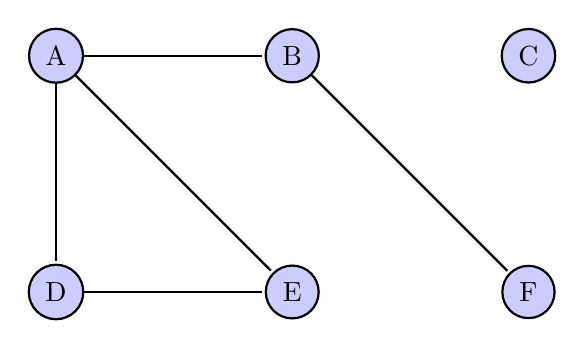
\begin{tikzpicture}[shorten >=1pt,auto,node distance=3cm,
  thick,main/.style={circle,fill=blue!20,draw}]
  			\node[main] (A) {A};
  			\node[main] (B) [right of=A] {B};
  			\node[main] (C) [right of=B] {C};
  			\node[main] (D) [below of=A] {D};
  			\node[main] (E) [right of=D] {E};
  			\node[main] (F) [right of=E] {F};
  			\path[every node/.style={font=\sffamily\small}]
  			(A) edge (B)
  			(A) edge (D)
  			(A) edge (E)
  			(D) edge (E)
  			(B) edge (F);
		\end{tikzpicture}
	\end{center}
	\begin{enumerate}
		\item What is the number of vertices in this graph?

		\begin{Freeform}{6}
		\Solution There are 6 vertices in this graph: $A, B, C, D, E, F$.	
		\end{Freeform}

		\item What is the number of edges in this graph?
		\begin{Freeform}{5}
		\Solution There are 5 edges in this graph: $\{A, B\}, \{A, D\}, \{D, E\}, \{A, E\}, \{B, F\}$.
		\end{Freeform}

		\item Which vertices are isolated?

		\begin{Multi}
		\begin{itemize}
		\FalseChoice\item $A$
		\FalseChoice\item $B$
		\TrueChoice\item $C$
		\FalseChoice\item $D$
		\FalseChoice\item $E$
		\FalseChoice\item $F$
		\end{itemize}
		\Hint Recall that an isolated vertex is one that has no edges incident on it.
		\Solution The only vertex with no edges attached to it is $C$.
		\end{Multi}
		
		\item What is the degree of the vertex $A$?
		\begin{Freeform}{3}
		\Hint Recall that the degree of a vertex is the number of edges incident on it.
		\Solution Vertex $A$ has $3$ edges incident on it, namely $\{A, B\}, \{A, D\}, \{A, E\}$.	
		\end{Freeform}

		\item What is the sequence of edges $\{D, A\}, \{A, B\}, \{B, F\}$? Check all that apply.
		\begin{Multi}
		\begin{itemize}
		\TrueChoice\item A simple path.
		\FalseChoice\item A cycle.
		\TrueChoice\item A walk.
		\FalseChoice\item A tour.
		\end{itemize}
		\Solution These $3$ edges form a path, because they are a sequence of edges, each starting from where the previous one ended. It is a simple path, because no vertex is visited more than once by following this path. A walk is more general than a simple path (repetition is allowed), and so any simple path is a walk as well. Finally we do not end the path at the vertex we started, so this is neither a tour nor a cycle.
		\end{Multi}
		
		\item What is the sequence of edges $\{D, A\}, \{A, E\}, \{E, D\}$? Check all that apply.
		\begin{Multi}
		\begin{itemize}
		\FalseChoice\item A simple path.
		\TrueChoice\item A cycle.
		\TrueChoice\item A walk.
		\TrueChoice\item A tour.
		\end{itemize}
		\Solution These $3$ edges form a cycle, because they are a sequence of edges, each starting from where the previous one ended and the last vertex is the same as the first one and no vertex is visited more than once. It is not a simple path, because simple paths cannot start and end at the same vertex. Walks and tours are both more general than cycles, so any cycle is both a walk and a tour as well.
		\end{Multi}
		
		\item What is the sequence of edges $\{B, F\}, \{F, B\}, \{B, A\}, \{A, B\}$? Check all that apply.
		\begin{Multi}
		\begin{itemize}
		\FalseChoice\item A simple path.
		\FalseChoice\item A cycle.
		\TrueChoice\item A walk.
		\TrueChoice\item A tour.
		\end{itemize}
		\Solution These $4$ edges form a tour, because they are a sequence of edges, each starting from where the previous one ended and the last vertex is the same as the first one. It is not a cycle because the vertex $B$ is visited twice. A walk is more general than a tour, so any tour is also a walk.
		\end{Multi}

		\item Is this graph connected?
		\begin{Choices}
		\begin{itemize}
		\FalseChoice\item Yes.
		\TrueChoice\item No.
		\end{itemize}
		\Hint Recall that a graph is connected if and only if there is at least one path between every two vertices.
		\Solution The graph is disconnected. The vertex $C$ is isolated. So it does not have any path to any other vertex.
		\end{Choices}

		\item How many connected components does this graph have?
		\begin{Freeform}{2}
		\Solution There are $2$ connected components. One is $\{A, B, D, E, F\}$	, and the other one is $\{C\}$.
		\end{Freeform}

	\end{enumerate}
	
	\item The following problems give you practice with directed graphs. Consider the directed graph pictured below.
	\begin{center}
		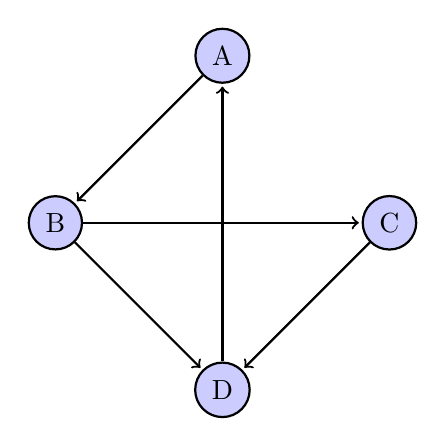
\begin{tikzpicture}[->, shorten >=1pt,auto,node distance=3cm,
  thick,main/.style={circle,fill=blue!20,draw}]
  			\node[main] (A) {A};
  			\node[main] (B) [below left of=A] {B};
  			\node[main] (C) [below right of=A] {C};
  			\node[main] (D) [below left of=C] {D};
  			\path[every node/.style={font=\sffamily\small}]
  			(A) edge (B)
  			(B) edge (C)
  			(C) edge (D)
  			(D) edge (A)
  			(B) edge (D);
		\end{tikzpicture}
	\end{center}
	\begin{enumerate}
		\item What is the out-degree of the vertex $D$?
		\begin{Freeform}{1}
		\Solution There is only one edge going out of $D$, namely $(D, A)$. So its out-degree is $1$.	
		\end{Freeform}

		\item What is the in-degree of the vertex $D$?
		\begin{Freeform}{2}
		\Solution There are two edges coming into $D$, namely $(B, D), (C, D)$. So its in-degree is $2$.
		\end{Freeform}
		
		\item Is the sequence of edges $(B, C), (C, D), (B, D)$ a tour?
		\begin{Choices}
		\begin{itemize}
		\FalseChoice\item Yes.
		\TrueChoice\item No.
		\end{itemize}
		\Solution No. This sequence of edges is not even a walk, because every edge must start from where the previous one ended. But $(B, D)$ does not start at $D$, where $(C, D)$ ended.
		\end{Choices}

		\item How many cycles does this graph have?
		\begin{Freeform}{2}
		\Solution There are $2$ cycles in this graph. One is $(A, B), (B, D), (D, A)$, and the other one is $(A, B), (B, C), (C, D), (D, A)$.	
		\end{Freeform}
		
		\item How many paths are there between $A$ and $D$?
		\begin{Freeform}{2}
		\Solution There are $2$ paths. One is $(A, B), (B, D)$, and the other one is $(A, B), (B, C), (C, D)$.
		\end{Freeform}
	\end{enumerate}
	
	\item In the following problem you will practice Eulerian tours. Consider the following graph.
	\begin{center}
		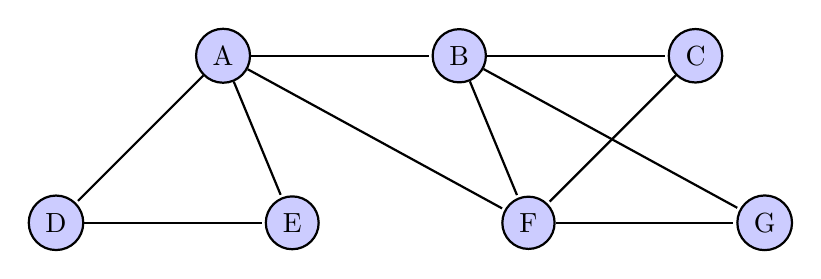
\begin{tikzpicture}[shorten >=1pt,auto,node distance=3cm,
  thick,main/.style={circle,fill=blue!20,draw}]
  			\node[main] (A) {A};
  			\node[main] (B) [right of=A] {B};
  			\node[main] (C) [right of=B] {C};
  			\node[main] (D) [below left of=A] {D};
  			\node[main] (E) [right of=D] {E};
  			\node[main] (F) [right of=E] {F};
  			\node[main] (G) [right of=F] {G};
  			\path[every node/.style={font=\sffamily\small}]
  			(A) edge (B)
  			(A) edge (D)
  			(A) edge (E)
  			(D) edge (E)
  			(B) edge (G)
  			(F) edge (G)
  			(B) edge (C)
  			(C) edge (F)
  			(B) edge (F)
  			(A) edge (F);
		\end{tikzpicture}
	\end{center}
	\begin{enumerate}
		\item Is this graph connected?
		\begin{Choices}
		\begin{itemize}
		\TrueChoice\item Yes.
		\FalseChoice\item No.
		\end{itemize}
		\Solution Yes. There is a path between every pair of vertices.
		\end{Choices}

		\item What is the set of degrees of vertices (after removing repetitions)?
		\begin{Choices}
		\begin{itemize}
		\FalseChoice\item $\{2, 4, 6\}$.
		\FalseChoice\item $\{4\}$
		\FalseChoice\item $\{2, 3, 4\}$.
		\TrueChoice\item $\{2, 4\}$.
		\FalseChoice\item $\{1, 2, 3, 4, 5\}$.
		\FalseChoice\item $\{2\}$.
		\end{itemize}
		\Solution The vertices $D, E, C$ are of degree $2$, and the vertices $A, B, F, G$ all have degree $4$. Therefore the set of degrees is $\{2, 4\}$.
		\end{Choices}

		\item If the set of degrees (after removing repetitions) of an imaginary graph is $\{2, 3, 4\}$, could it possibly have an Eulerian tour?
		\begin{Choices}
		\begin{itemize}
		\FalseChoice\item Yes.
		\TrueChoice\item No.
		\end{itemize}
		\Solution No. The degrees must all be even, so $3$ is not allowed if the graph is to have an Eulerian tour.
		\end{Choices}

		\item If the set of degrees (after removing repetitions) of an imaginary graph is $\{2, 4\}$, could it possibly have an Eulerian tour?
		\begin{Choices}
		\begin{itemize}
		\TrueChoice\item Yes.
		\FalseChoice\item No.
		\end{itemize}
		\Solution Yes. As long as the graph is connected, it will have an Eulerian tour, because all the degrees are even. And it is possible for such a graph to be connected (consider the example in this problem).
		\end{Choices}


		\item If the set of degrees (after removing repetitions) of an imaginary graph is $\{0, 2, 4\}$, could it possibly have an Eulerian tour?
		\begin{Choices}
		\begin{itemize}
		\TrueChoice\item Yes.
		\FalseChoice\item No.
		\end{itemize}
		\Solution Yes. The condition for having an Eulerian tour is having even degrees, and being connected, {\em except for isolated vertices}. Even though this graph is certainly disconnected, after removing isolated vertices, it could potentially be connected. Consider the example in this problem and add an isolated vertex to it. That would be a graph which still has an Eulerian tour, but has degree set $\{0, 2, 4\}$.
		\end{Choices}
		
		\item Now imagine that we want to find an Eulerian tour on the graph depicted in this problem. The first step is to run the procedure \textsc{FindTour} as defined in the lecture. Recall that this procedure starts at a vertex $v_0$, and from there chooses an arbitrary unexplored edge to go to $v_1$, and keeps on choosing unexplored edges until it returns to the original vertex. Obviously there are a lot of choices, and the tour that is found depends on them, so to make it unique let us always choose the unexplored edge that goes to the vertex which comes first alphabetically. If we run the procedure \textsc{FindTour} with the starting vertex $A$, what is the tour that is going to be found? Express your answer in this format: $[v_0\ v_1\ \dots\ v_n]$ where $v_0=A$ is the starting vertex and $v_n$ is the vertex you visit right before returning to $v_0$ (for example a potential answer might be $[A\ E\ D]$).
		\begin{Freeform}{[A B C F]}
		\Solution The answer is $[A\ B\ C\ F]$. After visiting $F$ the procedure returns back to $A$ and a tour is found.
		\end{Freeform}

		\item Let us call the tour that we just found $W$. After finding the tour $W$ and removing it from the graph, how many connected components remain that are not isolated vertices?
		\begin{Freeform}{2}
		\Solution Two connected components remain. They are $\{A, D, E\}$ and $\{B, F, G\}$.
		\end{Freeform}

		\item If we run the procedure \textsc{FindTour} in the connected component that contains $A$, again starting with $A$ and breaking ties alphabetically, what tour do we get? Express your answer in the same format as before.
		\begin{Freeform}{[A D E]}
		\Solution The tour that we get is $[A\ D\ E]$.
		\end{Freeform}
		
		\item If we run the procedure \textsc{FindTour} in the connected component that contains $B$, starting with $B$ and breaking ties alphabetically, what tour do we get? Express your answer in the same format as before.
		\begin{Freeform}{[B F G]}
		\Solution The tour that we get is $[B\ F\ G]$.	
		\end{Freeform}
		
		\item After finding these tours in the connected components, we now need to stitch them together with the help of the first tour ($W$) that we found. To do this, imagine that we are walking over $W$ in the same order as before (i.e. starting with $A$ and going to the alphabetically first neighbor for the first move). The first time we visit one of the vertices in one of the connected components that remain after removing $W$, we take a detour, by exploring the tour found in that connected component and returning back to our place, and then continuing the tour $W$. Assume that in each detour we walk in the same order as the answers you have reported (i.e. we move to the alphabetically first neighbor for the first step). This stitching procedure will give us the Eulerian tour. Report the resulting Eulerian tour in the same format as before (starting at $A$ and ending at the vertex right before the ending edge of the tour).
		\begin{Freeform}{[A D E A B F G B C F]} 
		\Hint The first detour is taken right at the beginning, and the second detour is taken right after walking over the first edge of $W$.
		\Solution Note that $W=[A\ B\ C\ F]$. So we start at $A$. Immediately we see that $A$ belongs to a connected component that results from the removal of $W$, so we take the detour $[A\ D\ E]$ and return back to $A$. Then we take the first edge of $W$ to $B$, and again we have to take a detour, i.e. $[B\ F\ G]$. Now we have taken all the necessary detours and we continue $W$ uninterrupted. The resulting Eulerian tour is $[A\ D\ E\ A\ B\ F\ G\ B\ C\ F]$.
		\end{Freeform}
	\end{enumerate}

	\item In the notes, you learn that a hypercube in $n$ dimensions is a graph in which each vertex corresponds to a binary string of length $n$, and each vertex is adjacent to all strings that differ from it in exactly one coordinate. For example, for $n = 3$, the vertex $(1,0,1)$ is adjacent to vertices $(1,0,0), (0,0,1)$, and $(1,1,1)$. 

	The hypercube is a graph in which each vertex has relatively low degree, and yet the graph is well-connected. That is, the number of edges that you need to remove in order to disconnect $k$ of the vertices from the other vertices is large (at least $k$, assuming $k\leq 2^{n-1}$).

	Here, we will build some intuition by working with examples. 
	\begin{enumerate}
		\item For $n = 2$, the hypercube is just a square. Examine the $2$-dimensional hypercube below.
		\begin{center}
		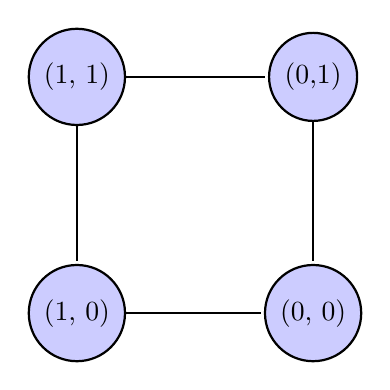
\begin{tikzpicture}[shorten >=1pt,auto,node distance=3cm, thick,main node/.style={circle,fill=blue!20,draw}]

			\node[main node] (1) {(1, 1)};
			\node[main node] (2) [below of=1] {(1, 0)};
			\node[main node] (3) [right of=1] {(0,1)};
			\node[main node] (4) [below of=3] {(0, 0)};

			\path[every node/.style={font=\sffamily\small}]
			(1) edge (2)
          		edge (3)
			(2) edge (4)
			(3) edge  (4);
		\end{tikzpicture}
		\end{center}
		\begin{enumerate}
			\item What is the degree of the vertices in this graph?
			\begin{Freeform}{2}
			$deg(v) =$ 
			\Hint How many neighbors does a vertex have in the $n$-dimensional hypercube?
			\Solution Each vertex has $2$ incident edges.
			\end{Freeform}
			
			\item What is the minimum number of edges $e$ you have to remove in order to make this graph disconnected?
			\begin{Freeform}{2}
			$e=$ 
			\Hint Look at the drawing. 
			\Solution We need at least $2$ edges. Removing any $1$ edge will leave us with a path of length $3$ which is connected.
			\end{Freeform}
		\end{enumerate}
		\item For $n = 3$, the hypercube is two squares connected by some edges. In fact, if you look below, you can see that we've chosen to highlight the square for which all boolean strings start with 1, and the square for which all boolean strings start with 0, as the subsquares.  Examine the $3$-dimensional hypercube below.
		\begin{center}
		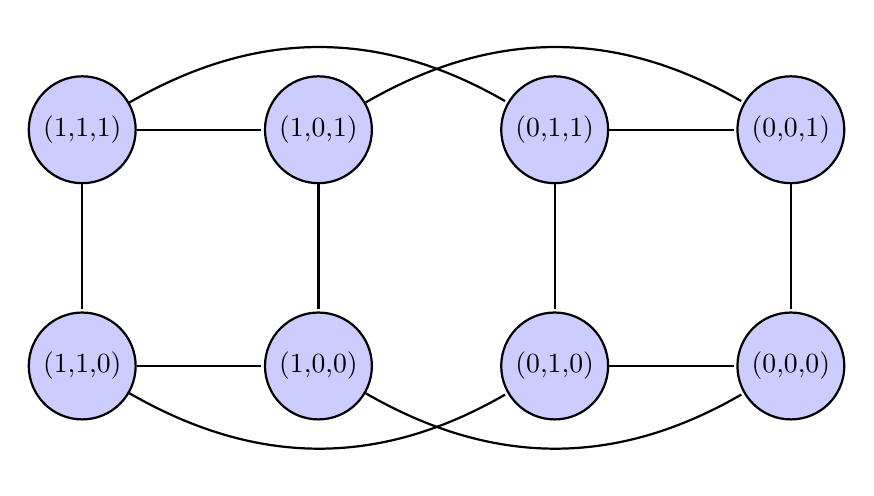
\begin{tikzpicture}[shorten >=1pt,auto,node distance=3cm, thick,main node/.style={circle,fill=blue!20,draw}]

			\node[main node] (1) {(1,1,1)};
			\node[main node] (2) [below of=1] {(1,1,0)};
			\node[main node] (3) [right of=1] {(1,0,1)};
			\node[main node] (4) [below of=3] {(1,0,0)};

			\node[main node] (5) [right of=3] {(0,1,1)};
			\node[main node] (6) [below of=5] {(0,1,0)};
			\node[main node] (7) [right of=5] {(0,0,1)};
			\node[main node] (8) [below of=7] {(0,0,0)};

			\path[every node/.style={font=\sffamily\small}]
			(1) edge (2)
          		edge (3)
			(2) edge (4)
			(3) edge (4)
			(5) edge (6)
				edge (7)
			(6) edge (8)
			(7) edge  (8)

			(1) edge [bend left] node [right] {} (5)
			(3) edge [bend left] node [right] {} (7)
			(2) edge [bend right] node [right] {} (6)
			(4) edge [bend right] node [right] {} (8);
		\end{tikzpicture}
		\end{center}
		\begin{enumerate}
			\item What is the degree of the vertices in this graph?
			\begin{Freeform}{3}
			$deg(v) =$ 
			\Hint How many neighbors does a vertex have in the $n$-dimensional hypercube?
			\Solution Each vertex has $3$ edges incident on it, corresponding to each of the $3$ bits.
			\end{Freeform}
			
			\item What is the minimum number of edges $e$ you have to remove in order to make this graph disconnected?
			\begin{Freeform}{3}
			$e=$ 
			\Hint Look at the drawing; what is the minimum number of edges you need to cut to separate vertex (1,1,1) from vertex (1,0,1)?
			\Solution We need $3$ edges. Again by looking at the picture one can see that no two edges would suffice.
			\end{Freeform}

			\item What was the ratio of (\# edges removed)/(\# vertices on the smaller side) in the previous part?
			\begin{Freeform}{3}
			ratio = 
			\Hint How many edges did you cut? How many vertices are left in the smaller side?
			\Solution We cut $3$ edges, separating $1$ vertex from the rest. So the ratio is $3$.
			\end{Freeform}

			\item What is the minimum number of edges $e$ you have to remove in order to separate the left square from the right square?
			\begin{Freeform}{4}
			$e=$ 
			\Hint Look at the drawing.
			\Solution There are $4$ edges going between these two, and we need to remove all of them.
			\end{Freeform}
			
			\item What was the ratio of (\# edges removed)/(\# vertices in smaller side) in the example in part iv?
			\begin{Freeform}{1}
			ratio = 
			\Hint How many edges did you remove? How many vertices are left in the smaller side?
			\Solution We removed $4$ edges, and both sides had $4$ vertices. Therefore the ratio is $1$.
			\end{Freeform}

		\end{enumerate}
		\vspace{0.5cm}
		Notice that the number of edges you had to remove is always at least equal to the number of vertices in the smaller side, post-removal. This is not true of graphs in general (see if you can think of a counterexample).\\

		If you want, try to generalize the trends you see here to the $n$-dimensional hypercube. Which edges should you remove in order to minimize the ratio of edges removed to size of the smaller piece? Which edges should you remove in order to minimize the ratio of edges removed to number of edges in the smaller piece? 
	\end{enumerate}
	
	\item In the following problems you will practice your knowledge about trees.
	\begin{enumerate}
		\item Which of the following graphs represent a tree?
		\begin{Multi}
		\begin{itemize}
			\FalseChoice\item 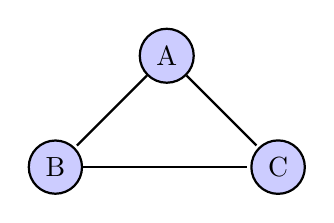
\begin{tikzpicture}[shorten >=1pt,auto,node distance=2cm, thick,main/.style={circle,fill=blue!20,draw}]
				\node[main] (A) {A};
				\node[main] (B) [below left of=A] {B};
				\node[main] (C) [below right of=A] {C};
				\path
				(A) edge (B)
					edge (C)
				(B) edge (C);
			\end{tikzpicture}
			\TrueChoice\item 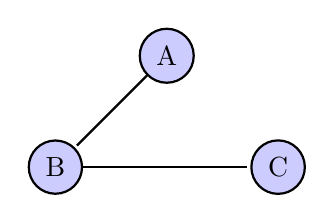
\begin{tikzpicture}[shorten >=1pt,auto,node distance=2cm, thick,main/.style={circle,fill=blue!20,draw}]
				\node[main] (A) {A};
				\node[main] (B) [below left of=A] {B};
				\node[main] (C) [below right of=A] {C};
				\path
				(A) edge (B)
				(B) edge (C);
			\end{tikzpicture}
			\FalseChoice\item 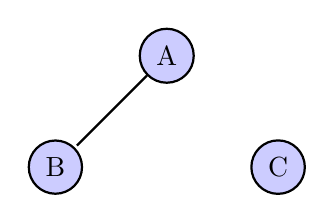
\begin{tikzpicture}[shorten >=1pt,auto,node distance=2cm, thick,main/.style={circle,fill=blue!20,draw}]
				\node[main] (A) {A};
				\node[main] (B) [below left of=A] {B};
				\node[main] (C) [below right of=A] {C};
				\path
				(A) edge (B);
			\end{tikzpicture}
			\TrueChoice\item 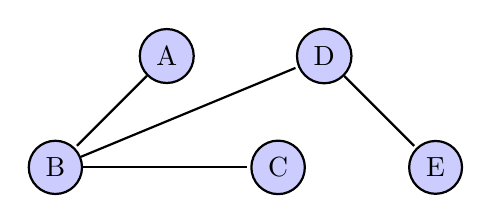
\begin{tikzpicture}[shorten >=1pt,auto,node distance=2cm, thick,main/.style={circle,fill=blue!20,draw}]
				\node[main] (A) {A};
				\node[main] (B) [below left of=A] {B};
				\node[main] (C) [below right of=A] {C};
				\node[main] (E) [right of=C] {E};
				\node[main] (D) [right of=A] {D};
				\path
				(A) edge (B)
				(B) edge (D)
				(B) edge (C)
				(D) edge (E);
			\end{tikzpicture}
		\end{itemize}
		\Hint Recall that a tree is a graph which has no cycles and is connected.
		\Solution A tree must have no cycles and be connected. The first graph has a cycle, and the third graph is not connected. The remaining two are trees.
		\end{Multi}

		\item How many edges does a tree that has $10$ vertices have?
		\begin{Freeform}{9}
			\Solution A tree with $n$ vertices has exactly $n-1$ edges.
		\end{Freeform}
		
		\item Consider the following rooted tree, which is rooted at $A$.
		\begin{center}
		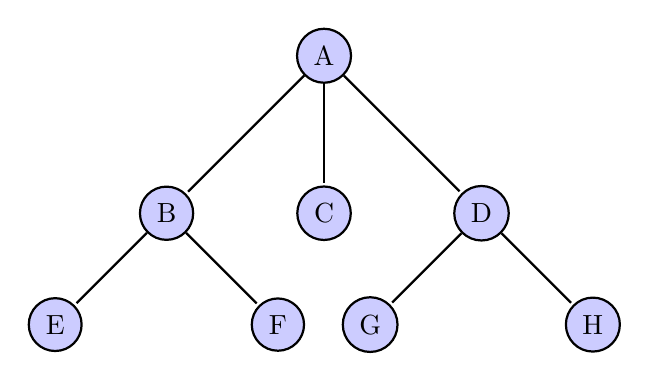
\begin{tikzpicture}[shorten >=1pt,auto,node distance=2cm, thick,main/.style={circle,fill=blue!20,draw}]
			\node[main] (A) {A};
			\node[main] (C) [below of=A] {C};
			\node[main] (B) [left of=C] {B};
			\node[main] (D) [right of=C] {D};
			\node[main] (E) [below left of=B] {E};
			\node[main] (F) [below right of=B] {F};
			\node[main] (G) [below left of=D] {G};
			\node[main] (H) [below right of=D] {H};
			\path
			(A) edge (B) edge (C) edge (D)
			(B) edge (E) edge (F)
			(D) edge (G) edge (H);
		\end{tikzpicture}
		\end{center}
		
		\begin{enumerate}
			\item Which of the following vertices are leaves?
			\begin{Multi}
			\begin{itemize}
			\FalseChoice\item $A$
			\TrueChoice\item $E$
			\FalseChoice\item $B$
			\TrueChoice\item $C$
			\TrueChoice\item $H$
			\end{itemize}
			\Hint Leaves are vertices that have only one edge attached to them.
			\Solution The leaves of this tree are $E, F, C, G, H$.
			\end{Multi}

			\item What is the depth of this tree?
			\begin{Freeform}{2}
			\Hint The depth is the length of the longest path from the root to any of the leaves.
			\Solution The longest path from the root to any of the leaves has length only $2$. One such path is the one between $A$ and $E$ (which passes through $B$).
			\end{Freeform}

			\item Which of the following are in level $1$ of this graph (note that level $0$ is just the root).
			\begin{Multi}
			\begin{itemize}
			\TrueChoice\item $B$
			\FalseChoice\item $E$
			\FalseChoice\item $A$
			\TrueChoice\item $C$
			\FalseChoice\item $H$
			\end{itemize}
			\Solution The vertices at level $1$ are $B, C, D$.
			\end{Multi}

		\end{enumerate}

	\end{enumerate}
	
	\item The following questions provide some practice about complete graphs.
	\begin{enumerate}
		\item How many edges are there in the complete graph on $5$ vertices ($K_5$)?
		\begin{Freeform}{10}
		\Solution In $K_n$ there are exactly $\frac{n(n-1)}{2}$ edges.	
		\end{Freeform}
		
		\item What is the degree of each vertex in $K_6$?
		\begin{Freeform}{5}
		\Solution In $K_n$ the degree of each vertex is exactly $n-1$, because it has edges to every single one of the other vertices.	
		\end{Freeform}

		\item Which of the following graphs have an Eulerian tour?
		\begin{Multi}
		\begin{itemize}
		\TrueChoice\item The complete graph on $5$ vertices ($K_5$).
		\FalseChoice\item The complete graph on $6$ vertices ($K_6$).
		\TrueChoice\item The complete graph on $7$ vertices ($K_7$).
		\FalseChoice\item The $3$-dimensional hypercube.
		\TrueChoice\item The $4$-dimensional hypercube.
		\end{itemize}
		\Hint A graph has an Eulerian tour if and only if its degrees are even and it is connected.
		\Solution Complete graphs and hypercubes are always connected. So it remains to check that they have even degrees. Vertices in the $d$-dimensional hypercube all have degree $d$; so hypercubes are Eulerian if and only if $d$ is even. In the complete graph on $n$ vertices, all vertices have degree $n-1$, so these graphs are Eulerian if and only if $n$ is odd.
		\end{Multi}
	\end{enumerate}

\end{enumerate}


\end{document}
